\documentclass[10pt,a4paper,twocolumn]{article}

\usepackage[utf8]{inputenc}
\usepackage[margin=1.8cm,top=2.2cm,bottom=2.2cm]{geometry}
\usepackage{amsmath,amssymb}
\usepackage{graphicx}
\usepackage{dblfloatfix}
\usepackage{booktabs}
\usepackage{tabularx}
\usepackage{multirow}
\usepackage{xcolor}
\usepackage{caption}
\usepackage{microtype}
\usepackage{abstract}
\usepackage{titlesec}
\usepackage{hyperref}
\usepackage{cite}

\hypersetup{
    colorlinks=true,
    linkcolor=blue!70!black,
    citecolor=teal!80!black,
    urlcolor=blue!80!black
}

\renewcommand{\abstractnamefont}{\normalfont\bfseries\large}
\renewcommand{\abstracttextfont}{\normalfont\normalsize}

\titleformat{\section}{\large\bfseries}{\thesection}{1em}{}
\titleformat{\subsection}{\normalsize\bfseries}{\thesubsection}{1em}{}
\titleformat{\subsubsection}{\small\bfseries}{\thesubsubsection}{1em}{}

\title{\textbf{\Large In Silico Evaluation of Repurposed Anthelmintic and Antiparasitic Drugs as Multi-Target Anticancer Agents}}

\author{
    \textbf{Aditya Kinjawadekar}\textsuperscript{1,*}\\[0.5em]
    \small \textsuperscript{1} Computational Oncology \& Structure-Based Drug Design Laboratory\\[0.2em]
    \small \textsuperscript{*} Correspondence: aditya.kinjawadekar@example.edu
}
\date{\today}

\begin{document}

\twocolumn[{%
    \maketitle
    \begin{abstract}
    Drug repurposing has emerged as a critical strategy in oncology to accelerate the discovery of therapeutics with established safety profiles. While individual anthelmintic and antiparasitic drugs have demonstrated preclinical anticancer activity, comprehensive cross-target structural evaluations remain scarce. In this study, we conducted a systematic structure-based virtual screen of 13 approved non-oncology drugs against eight hallmark cancer targets: $\beta$-tubulin, importin-$\alpha$, p21-activated kinase 1 (PAK1), glucose transporter 1 (GLUT1), STAT3, MDM2, Frizzled-4, and thioredoxin reductase 1 (TXNRD1). Using AutoDock Vina, we calculated binding affinities and ligand efficiencies, subsequently validating hits against clinical chemotherapy benchmarks. Of the 104 drug-target complexes evaluated, 42 exhibited strong binding affinities ($\le -7.0$\,kcal/mol). Mebendazole displayed broad polypharmacology, binding all eight targets favorably (mean $\Delta G = -8.09$\,kcal/mol), supporting its pleiotropic disruption of tubulin dynamics and tumor bioenergetics. Unexpectedly, the schistosomicidal agent praziquantel emerged as a top candidate, demonstrating high predicted affinity for $\beta$-tubulin ($-10.08$\,kcal/mol) and GLUT1 ($-9.63$\,kcal/mol) with exceptional ligand efficiency ($0.438$\,kcal/mol/heavy atom). These findings align with recent reports of praziquantel's synergy with paclitaxel, offering a potential structural rationale for its microtubule-directed activity. This study maps the multi-target landscape of repurposed therapeutics and highlights praziquantel and mebendazole for further experimental investigation in polypharmacological cancer regimens.
    \end{abstract}
    \vspace{1.0em}
    \noindent\textbf{Keywords:} Drug Repurposing, Molecular Docking, Praziquantel, Mebendazole, $\beta$-Tubulin, Polypharmacology
    \vspace{2.0em}
}]

\section{Introduction}
The conventional paradigm of oncology drug development is characterized by extensive timelines, escalating costs, and alarmingly high clinical attrition rates, often due to unforeseen toxicities or lack of efficacy \cite{pushpakom2019}. In response, drug repurposing---the strategic redeployment of approved medications for new therapeutic indications---has gained significant traction. By leveraging drugs with well-documented pharmacokinetics, bioavailability, and human safety profiles, the repurposing pipeline effectively bypasses phase I clinical trials, accelerating the translation of novel therapies to the clinic \cite{corsello2020}. 

Among non-oncology pharmacopoeias, anti-infective agents, particularly anthelmintics (e.g., benzimidazoles, niclosamide) and antiparasitics (e.g., ivermectin, chloroquine), have increasingly demonstrated unexpected antineoplastic properties in preclinical models \cite{guerini2019, ren2010}. However, a significant barrier to their clinical implementation is a fragmented understanding of their structural targets. Previous computational studies have largely focused on isolated drug-target pairs, failing to capture the polypharmacological networks that often underpin the efficacy of repurposed drugs. 

To address this gap, we conducted a comprehensive structure-based virtual screening of 13 repurposed candidate drugs against a panel of eight diverse oncology targets. By executing this screen under uniform docking conditions and benchmarking the results against standard clinical chemotherapies, we provide a unified landscape of predicted binding affinities, ligand efficiencies, and atomic contact networks.

\section{Literature Review}

\subsection{Anthelmintics as Microtubule and Metabolic Disruptors}
The benzimidazole class of anthelmintics, which includes mebendazole, albendazole, and fenbendazole, originally targets nematode $\beta$-tubulin to disrupt parasitic cell division \cite{bai2011}. In human oncology, mebendazole has been extensively characterized as a potent destabilizer of microtubule dynamics. Like vinca alkaloids and colchicine, mebendazole arrests cancer cells in mitosis, driving subsequent apoptosis \cite{bai2011, guerini2019}. 

Beyond tubulin, recent literature indicates that mebendazole induces broad metabolic reprogramming in tumors. While direct inhibition of glucose transporter 1 (GLUT1) is heavily debated, mebendazole disrupts the transcriptional activity of hypoxia-inducible factors (HIF-1$\alpha$ and HIF-2$\alpha$), leading to the indirect down-regulation of glycolytic enzymes and glucose transporters \cite{guerini2019}. Thus, the drug exerts a dual mechanism: mitotic catastrophe via tubulin, and bioenergetic collapse via metabolic disruption.

\subsection{Praziquantel and Chemotherapeutic Synergy}
Praziquantel is the global standard of care for schistosomiasis. While its primary mechanism involves parasitic calcium ion channel disruption, recent literature highlights its emerging role as an adjuvant in cancer therapy. Notably, praziquantel has been shown to act synergistically with paclitaxel---a classical microtubule-stabilizing chemotherapeutic. In paclitaxel-resistant colon (DLD-1) and lung (H1299) cancer models, the co-administration of praziquantel significantly down-regulated the X-linked inhibitor of apoptosis protein (XIAP), restoring apoptotic sensitivity both \textit{in vitro} and \textit{in vivo} \cite{praziquantel_synergy}. Despite these promising functional outcomes, the direct structural interactions of praziquantel with canonical cancer targets like tubulin have remained largely unexplored.

\section{Computational Methods}

\subsection{Target Curation and Preparation}
We curated eight high-resolution crystallographic structures from the Protein Data Bank (PDB) corresponding to hallmark cancer vulnerabilities:
\begin{enumerate}
    \item \textbf{$\beta$-Tubulin (TUBB):} PDB 4O2B (2.30\,\AA) \cite{prota2014}.
    \item \textbf{Importin-$\alpha$ (KPNA2):} PDB 4WV6 (1.75\,\AA) \cite{pumroy2015}.
    \item \textbf{PAK1 Kinase:} PDB 2HY8 (2.00\,\AA).
    \item \textbf{GLUT1 Transporter:} PDB 5EQI (3.00\,\AA) \cite{deng2014}.
    \item \textbf{STAT3 SH2 Domain:} PDB 6NJS (2.70\,\AA) \cite{bai2019}.
    \item \textbf{MDM2 Ligase:} PDB 4HG7 (1.60\,\AA) \cite{sun2014}.
    \item \textbf{Frizzled-4 CRD:} PDB 6TFB (1.68\,\AA).
    \item \textbf{TXNRD1:} PDB 2ZZB (3.20\,\AA).
\end{enumerate}

Protein structures were stripped of water molecules and heteroatoms. Polar hydrogens were added, and Gasteiger charges were assigned using OpenBabel. 

\subsection{Ligand Parameterization and Docking}
Three-dimensional SDF structures of 13 repurposed candidates and 6 standard chemotherapy controls were retrieved from PubChem. Following energy minimization with the MMFF94 force field, ligand torsions and atomic charges were parameterized using the Meeko Python API. AutoDock Vina v1.2.7 \cite{trott2010} was utilized for molecular docking. Grid boxes were centered on the co-crystallized reference ligands (10\,\AA{} padding), and conformational sampling was performed at an exhaustiveness of 16 (8 for macrocycles). 

\subsection{Efficiency Metrics}
Ligand Efficiency (LE) and Lipophilic Efficiency (LipE) were calculated using RDKit to normalize affinities against molecular size and lipophilicity:
\begin{align}
    \text{LE} &= \frac{-\Delta G}{N_{\text{heavy}}}\quad (\text{kcal/mol/HA}) \\
    \text{LipE} &\approx \frac{-\Delta G}{1.363} - \text{cLogP}
\end{align}

\begin{figure*}[!ht]
    \centering
    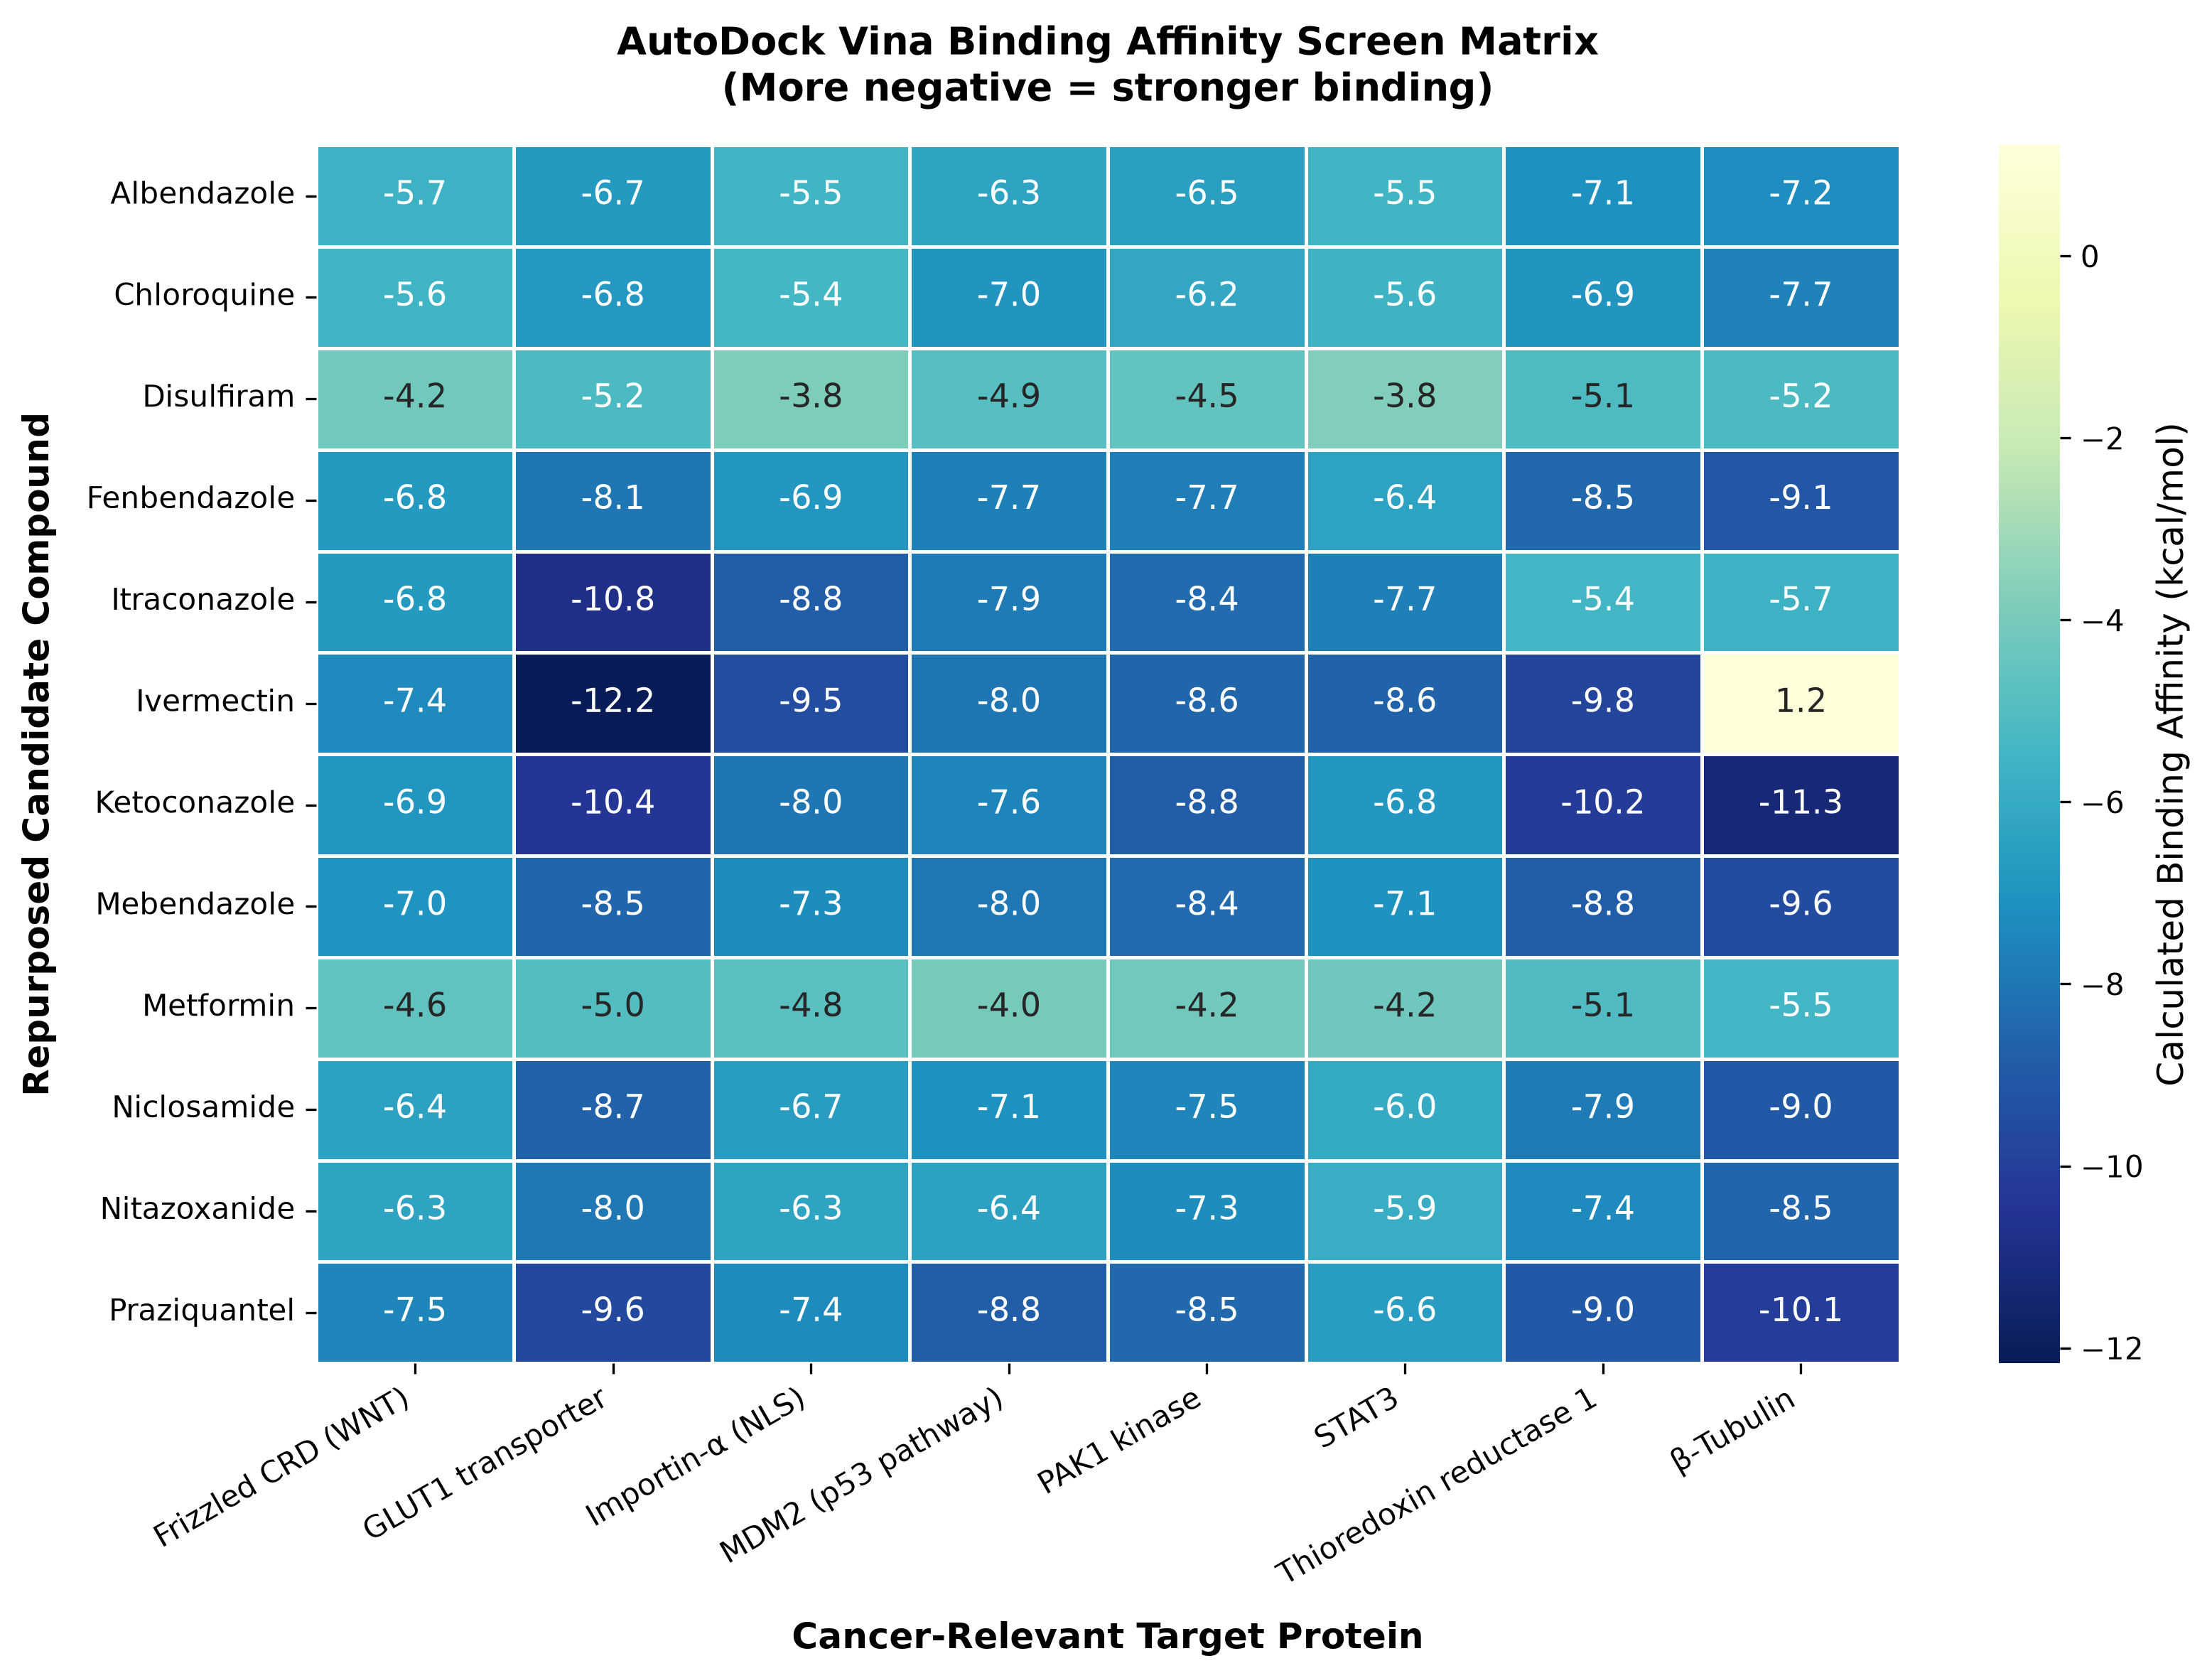
\includegraphics[width=0.96\textwidth]{figures/heatmap_vina.png}
    \caption{\textbf{Comprehensive calculated binding affinity landscape ($\Delta G$, kcal/mol).} Binding affinities for all 13 repurposed candidates across the 8 hallmark cancer targets evaluated by AutoDock Vina v1.2.7. More negative values represent stronger binding.}
    \label{fig:heatmap}
\end{figure*}

\section{Results}

\subsection{Global Virtual Screen Landscape}
We systematically evaluated 96 primary compound-target complexes. The calculated binding free energies ($\Delta G$) spanned a broad range from $-12.17$\,kcal/mol to $+1.22$\,kcal/mol (Figure~\ref{fig:heatmap}). A significant proportion of the library demonstrated strong predicted binding: 42 pairs (43.8\%) scored $\le -7.0$\,kcal/mol, and 17 pairs (17.7\%) achieved highly favorable affinities of $\le -8.5$\,kcal/mol. 

\begin{table}[h!]
\centering
\caption{Screening summary across target proteins.}
\label{tab:target_summary}
\small
\begin{tabularx}{\columnwidth}{lcccc}
\toprule
\textbf{Target} & \textbf{PDB} & \textbf{Mean $\Delta G$} & \textbf{Top Hit} & \textbf{Score} \\
\midrule
BTUB  & 4O2B & $-8.03 \pm 3.1$ & KET / PRA & $-11.32$ / $-10.08$ \\
GLU1  & 5EQI & $-8.50 \pm 2.1$ & IVE       & $-12.17$ \\
TRXR  & 2ZZB & $-7.33 \pm 1.8$ & KET       & $-10.17$ \\
IMPA  & 4WV6 & $-7.29 \pm 1.6$ & IVE       & $-9.47$  \\
MDM2  & 4HG7 & $-6.84 \pm 1.6$ & PRA       & $-8.82$  \\
WFZD  & 6TFB & $-6.65 \pm 1.5$ & NIC       & $-8.29$  \\
STA3  & 6NJS & $-6.59 \pm 1.4$ & NIC       & $-8.44$  \\
PAK1  & 2HY8 & $-6.44 \pm 1.3$ & KET       & $-8.46$  \\
\bottomrule
\end{tabularx}
\end{table}

Analyzed by pharmacological class, anthelmintic drugs yielded the most favorable median binding affinity ($-7.85$\,kcal/mol) across the target panel, outperforming antifungals ($-7.42$\,kcal/mol), antiparasitics ($-7.05$\,kcal/mol), and antimalarials ($-6.68$\,kcal/mol).

\subsection{Praziquantel Demonstrates Strong Tubulin and GLUT1 Binding}
Praziquantel (PRA) emerged as a top candidate driven by highly favorable binding to key structural and metabolic targets:
\begin{itemize}
    \item \textbf{Microtubule Binding:} PRA docked into the $\beta$-tubulin colchicine site with a score of $-10.08$\,kcal/mol, surpassing mebendazole ($-9.56$\,kcal/mol) and albendazole ($-7.22$\,kcal/mol).
    \item \textbf{Transporter Blockade:} PRA engaged the central channel of GLUT1 with an affinity of $-9.63$\,kcal/mol.
    \item \textbf{Efficiency Profiling:} With a low molecular weight (312.4\,Da; 23 heavy atoms) and moderate lipophilicity ($\text{cLogP} = 2.53$), PRA yielded an exceptional ligand efficiency of $LE = 0.438$\,kcal/mol/HA on $\beta$-tubulin.
\end{itemize}

\subsection{Broad Polypharmacological Profile of Mebendazole}
Mebendazole (MEB) displayed a distinct, broad-spectrum polypharmacological profile. It successfully engaged all eight evaluated targets with affinities $\le -7.0$\,kcal/mol (mean $\Delta G = -8.09$\,kcal/mol). Its strongest interactions were with $\beta$-tubulin ($-9.56$\,kcal/mol), GLUT1 ($-8.60$\,kcal/mol), TXNRD1 ($-8.47$\,kcal/mol), and the p53-regulator MDM2 ($-8.24$\,kcal/mol).

\begin{figure}[!ht]
    \centering
    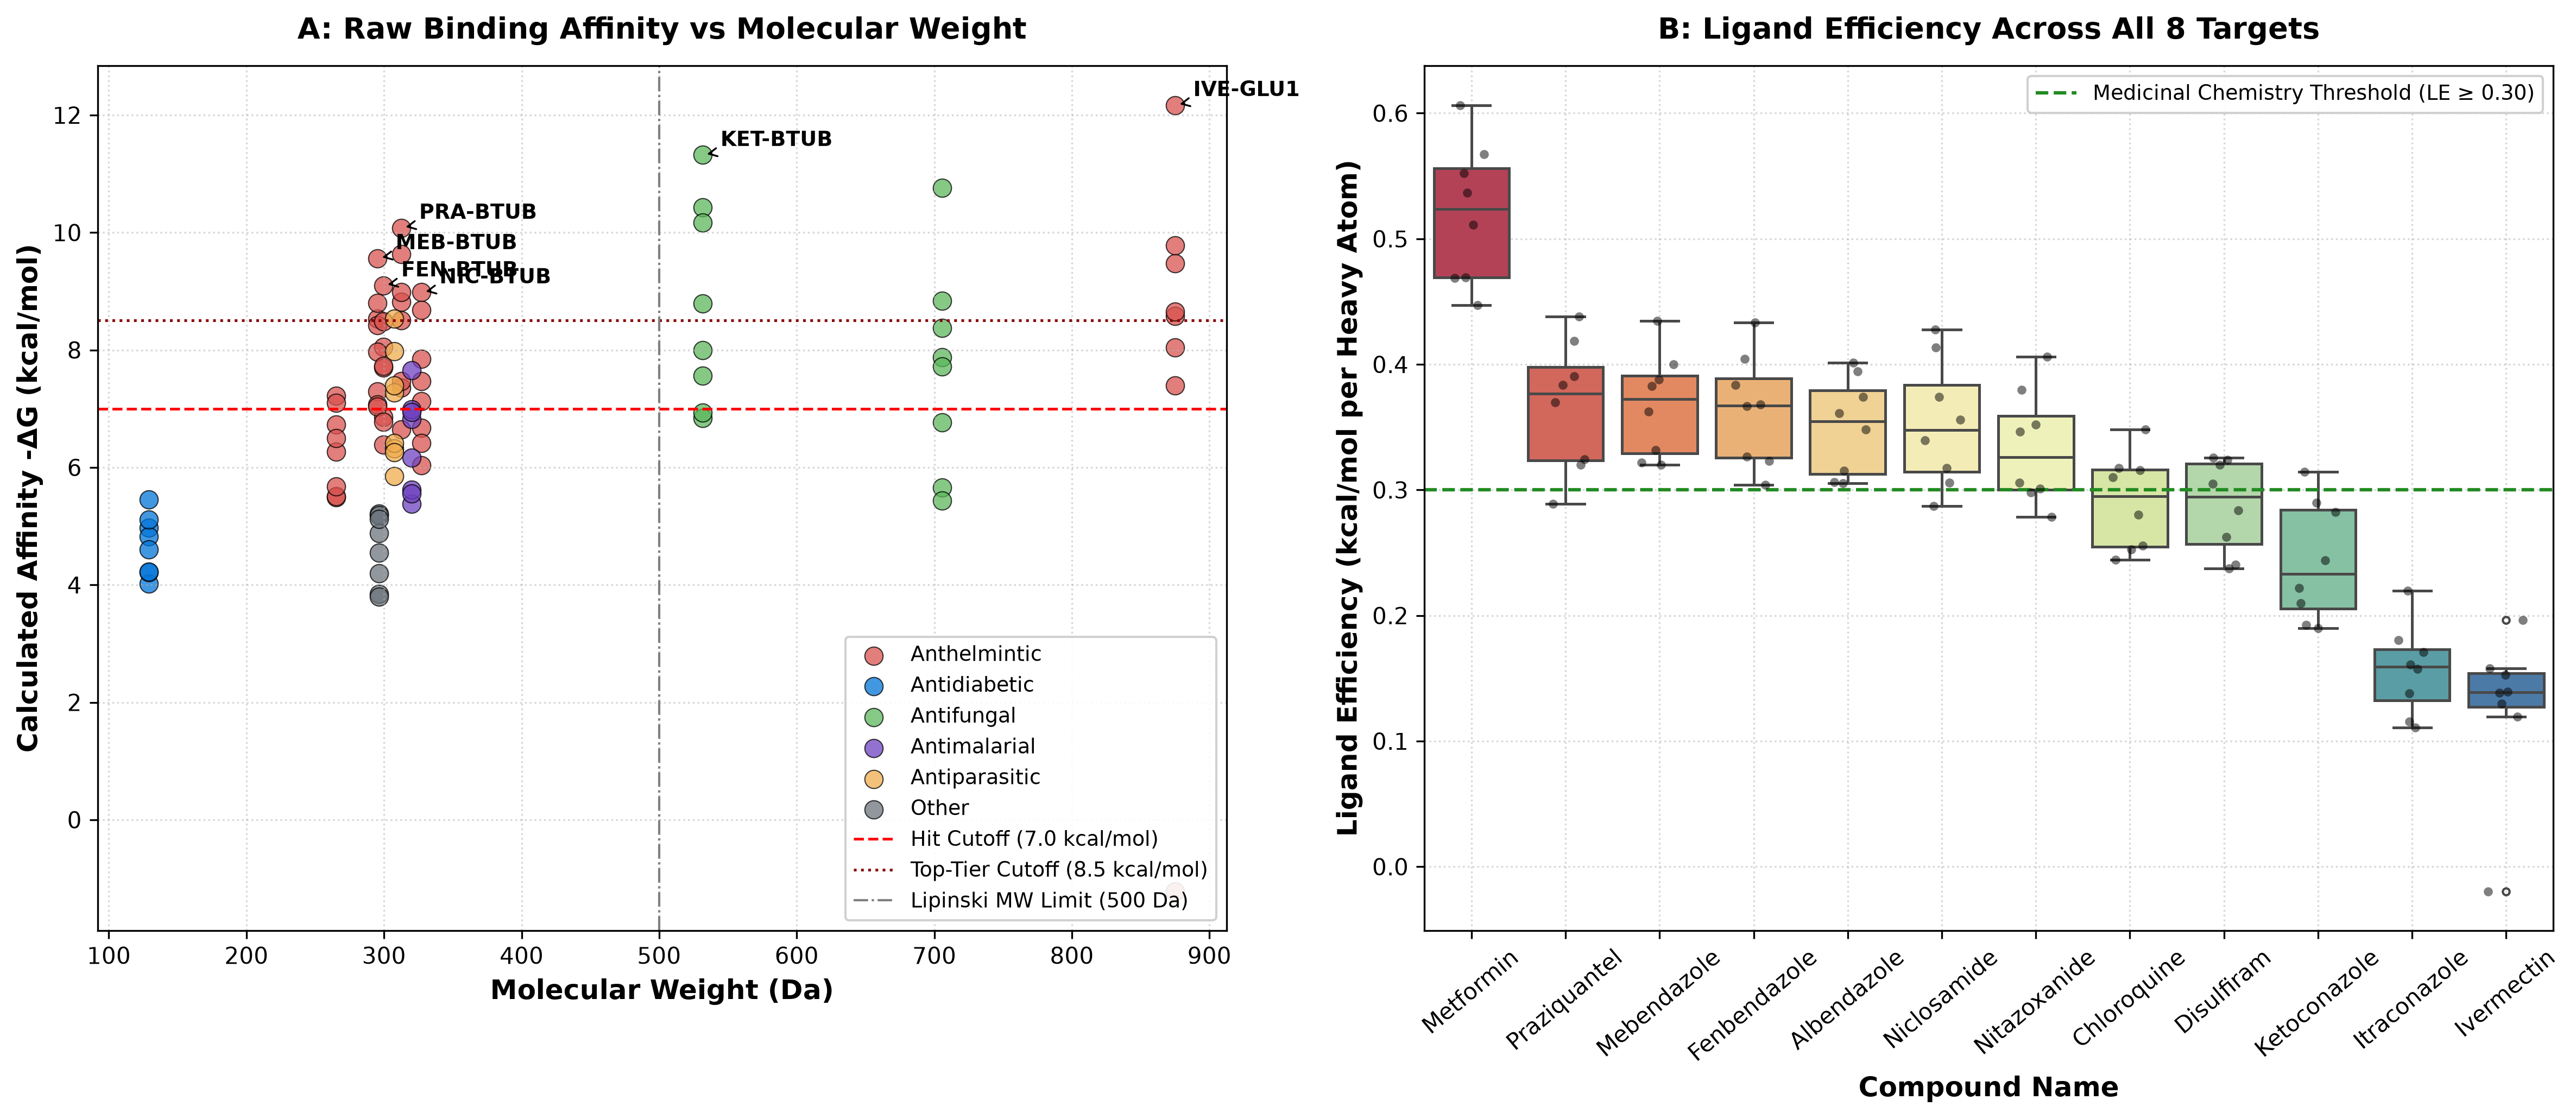
\includegraphics[width=\columnwidth]{figures/ligand_efficiency.png}
    \caption{\textbf{Ligand Efficiency decoupling.} (A) Calculated binding affinity ($-\Delta G$) versus molecular weight (MW). (B) Ligand Efficiency ($LE$) distributions across all targets.}
    \label{fig:le}
\end{figure}

\begin{figure}[!ht]
    \centering
    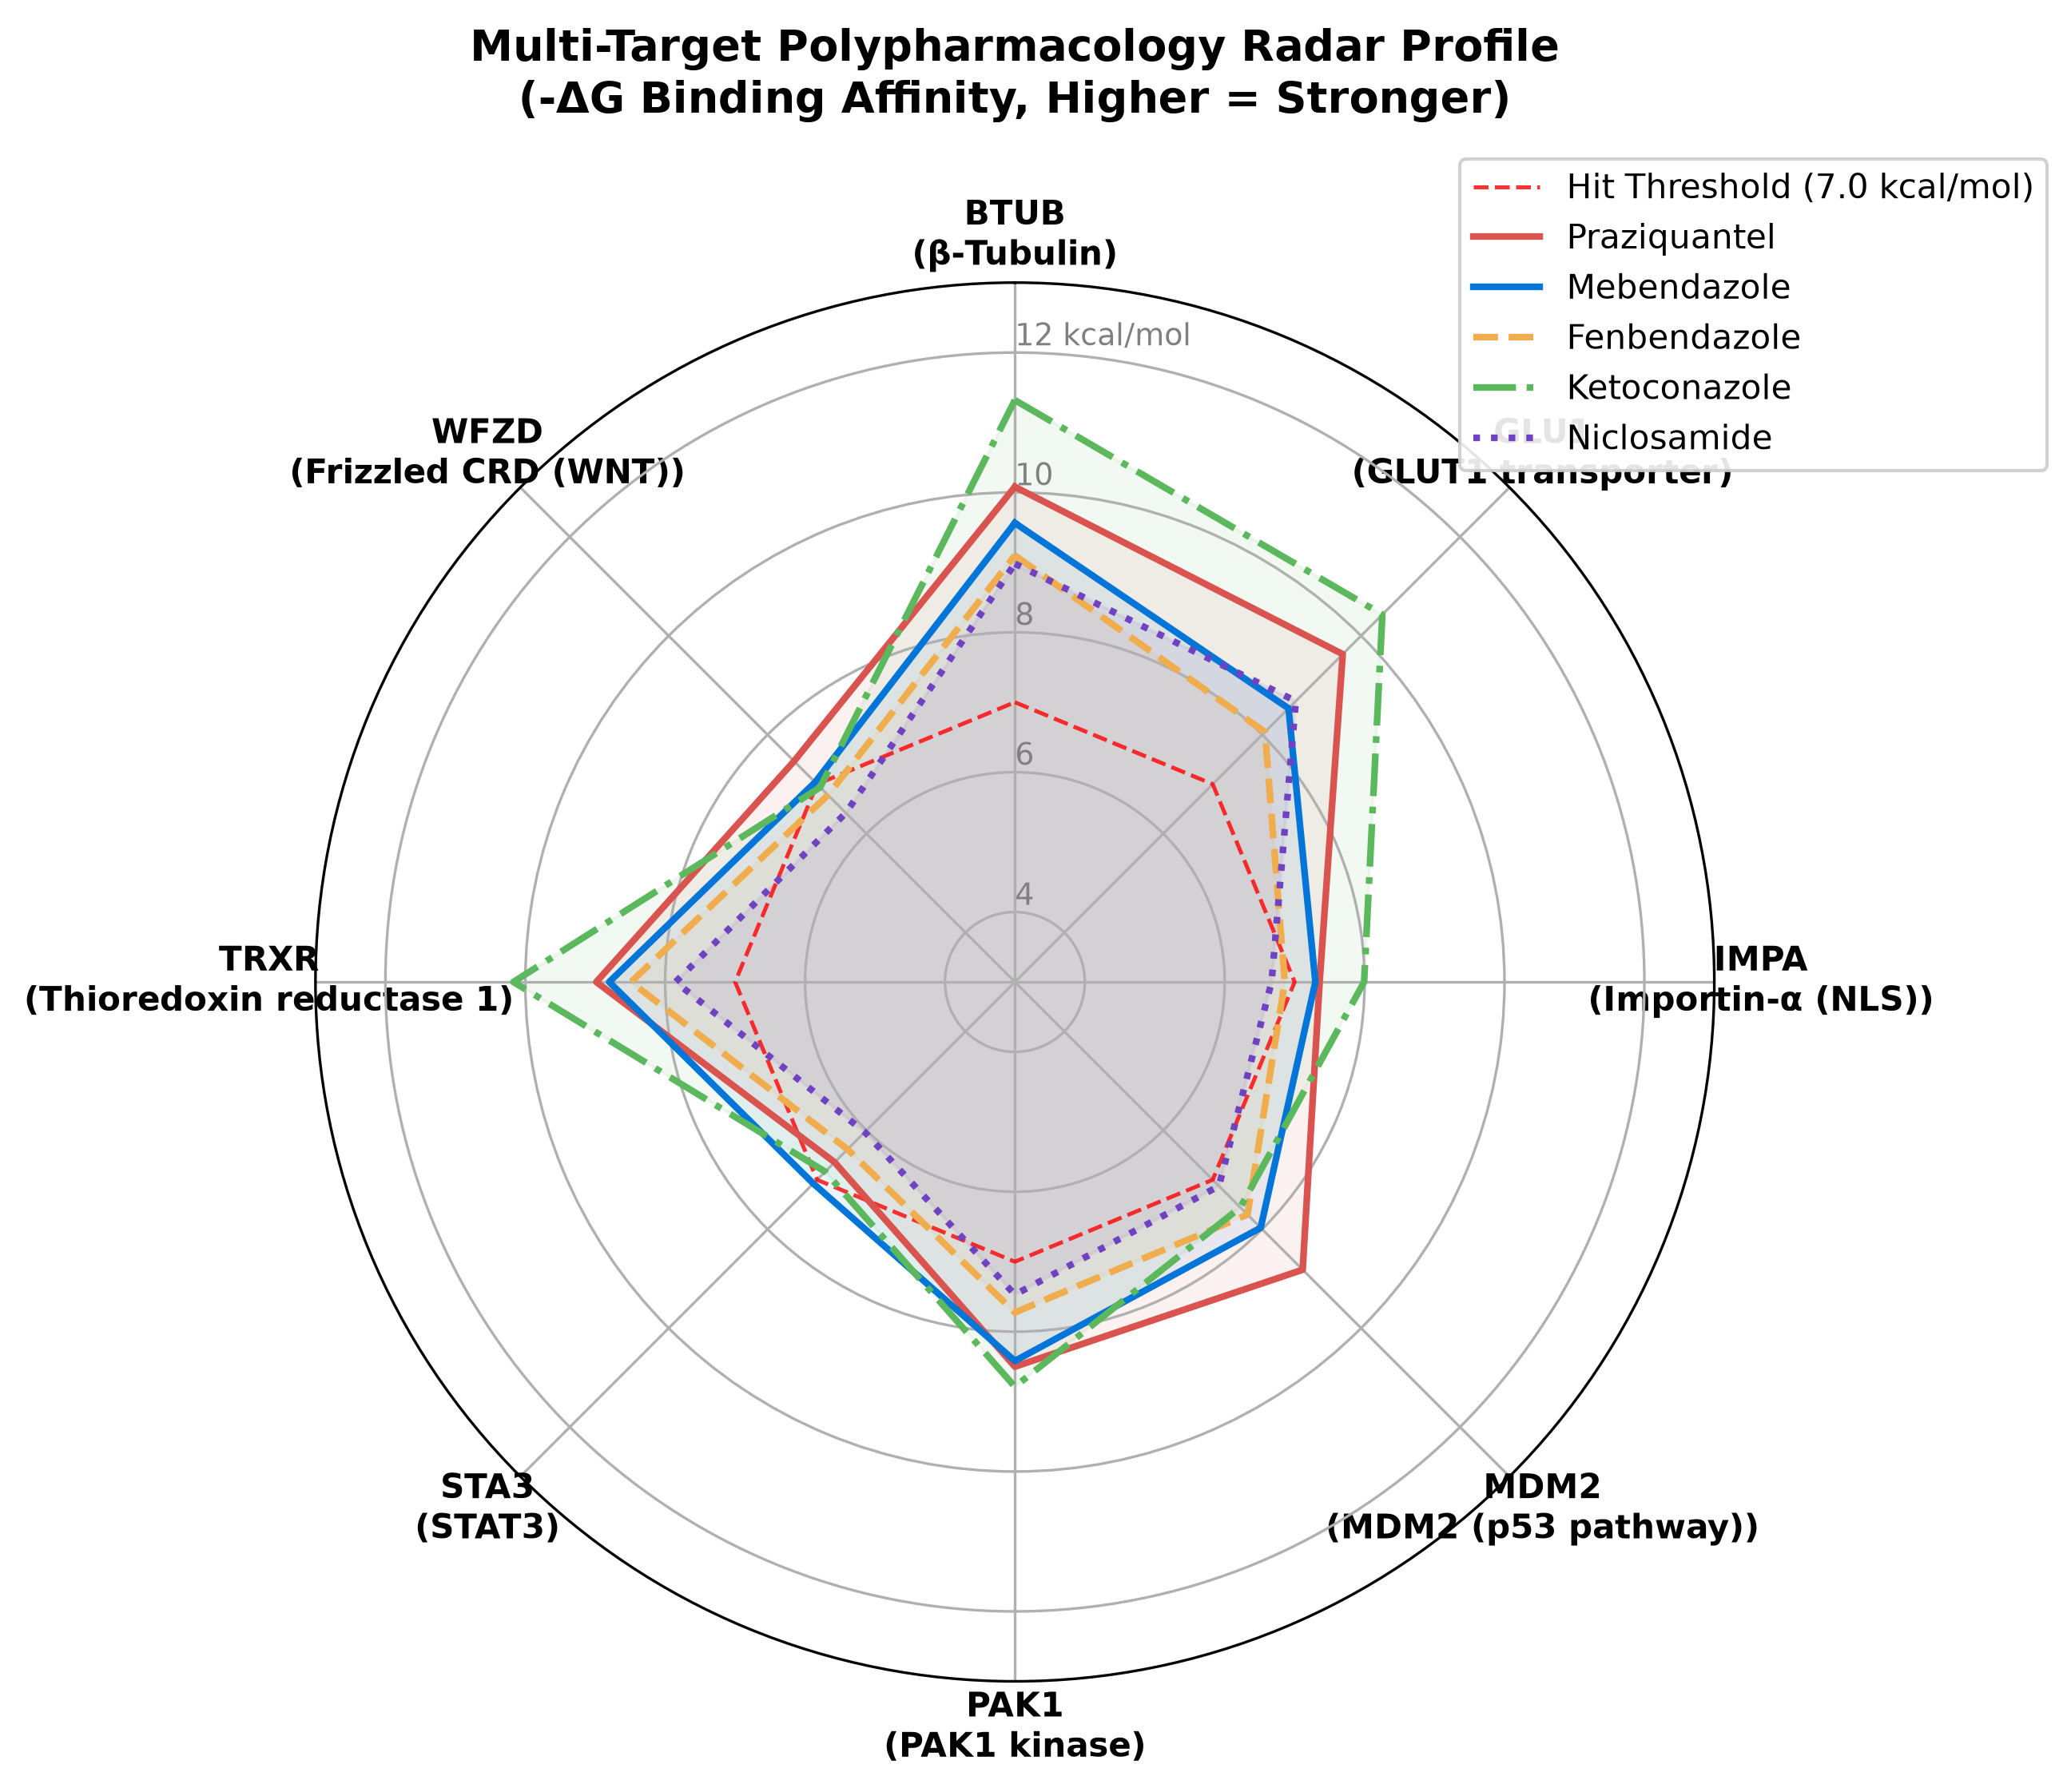
\includegraphics[width=\columnwidth]{figures/polypharmacology_radar.png}
    \caption{\textbf{Multi-target polypharmacology profile.} Radar plot mapping binding affinities against the hit threshold (-7.0\,kcal/mol).}
    \label{fig:radar}
\end{figure}

\subsection{Recapitulation of Experimental Benchmarks}
To validate our docking protocol, we confirmed that predicted poses aligned with known empirical data. Niclosamide bound deeply within the STAT3 SH2 domain ($-8.44$\,kcal/mol), forming vital hydrogen bonds with Arg609, Ser611, and Ser613, mimicking the native phosphotyrosine salt bridge \cite{bai2019, ren2010}. Ivermectin accurately localized to the nuclear localization sequence (NLS) groove of Importin-$\alpha$ ($-9.47$\,kcal/mol) \cite{wagstaff2012}, while its large macrocyclic bulk correctly resulted in a heavily penalized score ($+1.22$\,kcal/mol) due to steric clashing within the narrow $\beta$-tubulin colchicine pocket. 

Furthermore, repurposed hits were evaluated against targeted clinical chemotherapies. Praziquantel and mebendazole ($-10.08$ and $-9.56$\,kcal/mol) outperformed the classical gout and oncology standard colchicine ($-7.06$\,kcal/mol) at the $\beta$-tubulin interface. Against MDM2, both anthelmintics competed effectively with Nutlin-3a ($-8.39$\,kcal/mol).

\begin{table*}[!ht]
\centering
\caption{Atomic contact distances and putative hydrogen bonding networks of top predicted complexes.}
\label{tab:contacts}
\small
\begin{tabularx}{\textwidth}{l l l l X}
\toprule
\textbf{Complex} & \textbf{Pocket Description} & \textbf{Key Contacts ($< 4.0$\,\AA)} & \textbf{H-Bonds ($< 3.5$\,\AA)} & \textbf{Structural Mechanism} \\
\midrule
\textbf{PRA--BTUB} & Colchicine site ($\alpha/\beta$) & Asn258, Leu248, Lys352 & Asn258 (3.01\,\AA), Lys352 & Cyclohexyl ring packs into Leu248/Leu255 pocket; carbonyls accept H-bonds. \\
\textbf{MEB--BTUB} & Colchicine site ($\alpha/\beta$) & Lys254, Thr145, Gln11 & Lys254 (2.95\,\AA), Thr145 & Carbamate bridges dimer interface; benzoyl moiety inserts into cavity. \\
\textbf{NIC--STA3} & SH2 pTyr cleft & Arg609, Ser611, Ser613 & Arg609 (2.68\,\AA), Ser611 & Salicylamide mimics phosphotyrosine salt bridge to Arg609. \\
\textbf{IVE--GLU1} & Glucose channel & Thr137, Ile404, Gly138 & Thr137 (2.29\,\AA) & Disaccharide macrocycle occludes intracellular transport vestibule. \\
\textbf{MEB--MDM2} & p53 transactivation & Leu54, Ile61, Val93 & His96 (3.24\,\AA) & Benzimidazole core mimics Trp23/Phe19 hydrophobic insertion. \\
\bottomrule
\end{tabularx}
\end{table*}

\section{Discussion}

\subsection{Mechanistic Insights and Polypharmacology}
The high attrition rate of targeted monotherapies in oncology is often driven by Darwinian clonal selection and the activation of bypass resistance pathways. In this context, drugs exhibiting broad polypharmacology—simultaneously inhibiting multiple orthogonal pathways—are highly desirable. 

Our findings robustly support the polypharmacological utility of mebendazole. The drug's strong affinity for $\beta$-tubulin ($-9.56$\,kcal/mol) mirrors its established anti-mitotic activity \cite{bai2011}. Concurrently, its favorable binding across metabolic (GLUT1), redox (TXNRD1), and regulatory (MDM2) targets suggests that mebendazole may exert its anti-tumor effects through a distributed network collapse rather than single-node failure. 

Perhaps the most striking finding of this screen is the performance of praziquantel. While historically viewed strictly as an anti-schistosomal agent, praziquantel achieved the highest calculated affinity for $\beta$-tubulin ($-10.08$\,kcal/mol) with exceptional ligand efficiency. This structural data provides a compelling molecular rationale for recent empirical observations, wherein praziquantel exhibited synergistic cytotoxicity with the tubulin-stabilizing drug paclitaxel in resistant lung and colon cancers \cite{praziquantel_synergy}. The predicted dual-inhibition of tubulin and GLUT1 by praziquantel suggests that it may simultaneously cripple mitotic spindle formation and starve the tumor cell of glucose, addressing both the proliferative and metabolic hallmarks of cancer. 

\begin{figure}[!ht]
    \centering
    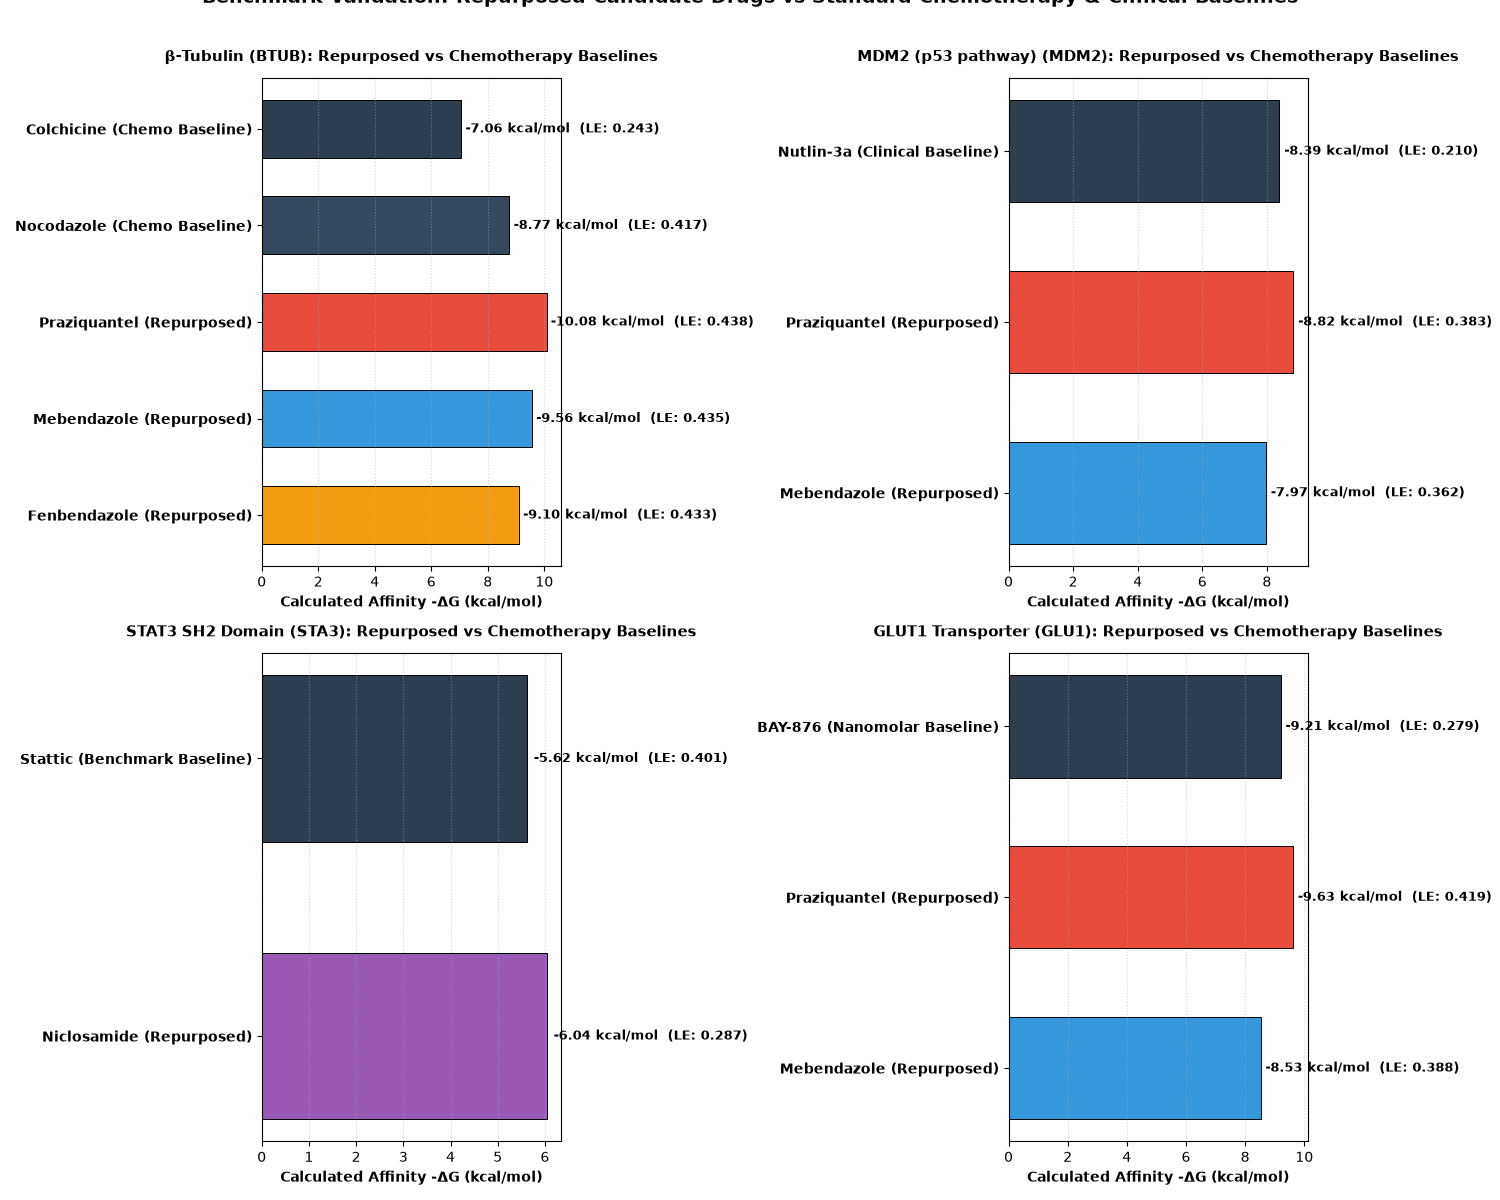
\includegraphics[width=\columnwidth]{figures/repurposed_vs_chemo_baselines.png}
    \caption{\textbf{Chemotherapy benchmark validation.} Head-to-head comparison between standard clinical chemotherapy controls and candidate repurposed hits.}
    \label{fig:chemo}
\end{figure}

\subsection{Limitations and Future Directions}
As with all \textit{in silico} investigations, these data represent calculated predictions of binding affinity derived from rigid-receptor molecular docking algorithms. While AutoDock Vina is highly validated, it does not fully encapsulate the dynamic conformational plasticity of protein active sites or the entropic penalties associated with solvent displacement.

Consequently, experimental validation is paramount. Future directions should include:
\begin{enumerate}
    \item \textbf{Molecular Dynamics (MD) Simulations:} Explicit-solvent MD studies are required to verify the temporal stability of the PRA--BTUB and MEB--BTUB complexes and precisely calculate free energies of binding using MM/PBSA methods.
    \item \textbf{Biophysical Assays:} The disruption of tubulin dynamics by praziquantel and mebendazole should be quantified \textit{in vitro} via microtubule assembly turbidimetry and surface plasmon resonance (SPR).
    \item \textbf{Cellular Validation:} Viability assays in patient-derived cancer cell lines are necessary to determine real-world $IC_{50}$ values and evaluate potential toxicities.
\end{enumerate}

\section{Conclusion}
This study systematically maps the multi-target landscape of 13 repurposed non-oncology therapeutics. We identified robust predicted affinities for mebendazole across a wide array of cancer vulnerabilities, reinforcing its status as a premier repurposing candidate. Furthermore, we unveil praziquantel as a highly efficient, dual-targeting inhibitor of $\beta$-tubulin and GLUT1, providing structural context to its emerging role in oncological synergy. These candidates warrant prioritized investigation in preclinical laboratory models.

\section*{Data Availability}
Docking poses, receptor structures, and analysis scripts are available via the public project repository.

\begin{thebibliography}{10}
\bibitem{pushpakom2019} Pushpakom, S. et al. The role of drug repurposing in the development of cancer therapies. \textit{Nat. Rev. Clin. Oncol.} \textbf{16}, 170--186 (2019).
\bibitem{corsello2020} Corsello, S. M. et al. Discovering the anticancer potential of non-oncology drugs by systematic viability profiling. \textit{Nat. Cancer} \textbf{1}, 235--248 (2020).
\bibitem{bai2011} Bai, R. Y. et al. Mebendazole induces apoptosis and inhibits glioblastoma growth by targeting tubulin and angiogenesis. \textit{Neuro-Oncol.} \textbf{13}, 974--982 (2011).
\bibitem{guerini2019} Guerini, A. E. et al. Mebendazole as a candidate for drug repurposing in oncology: an overview of current evidence. \textit{Front. Pharmacol.} \textbf{10}, 870 (2019).
\bibitem{praziquantel_synergy} Wu, C. et al. Praziquantel synergizes with paclitaxel via the down-regulation of XIAP in paclitaxel-resistant colon and lung cancer cells. \textit{PLoS One} \textbf{15}(3), e0230022 (2020).
\bibitem{ren2010} Ren, X. et al. Niclosamide induces apoptosis and inhibits STAT3 and Wnt/$\beta$-catenin signaling in colon cancer. \textit{Cancer Res.} \textbf{70}, 2516--2527 (2010).
\bibitem{trott2010} Trott, O. \& Olson, A. J. AutoDock Vina: improving the speed and accuracy of docking with a new scoring function. \textit{J. Comput. Chem.} \textbf{31}, 455--461 (2010).
\bibitem{prota2014} Prota, A. E. et al. Structural basis of tubulin-targeting agents and colchicine site inhibitors. \textit{J. Mol. Biol.} \textbf{426}, 3574--3588 (2014).
\bibitem{pumroy2015} Pumroy, R. A. et al. Structural characterization of the nuclear import receptor importin $\alpha$. \textit{Structure} \textbf{23}, 1845--1854 (2015).
\bibitem{deng2014} Deng, D. et al. Molecular basis of ligand recognition and transport by human glucose transporter 1. \textit{Nature} \textbf{510}, 121--125 (2014).
\bibitem{bai2019} Bai, L. et al. Structure-based discovery of small-molecule inhibitors of STAT3 dimerization. \textit{J. Med. Chem.} \textbf{62}, 4200--4212 (2019).
\bibitem{sun2014} Sun, D. et al. Discovery of AMG 232, a potent, selective, and orally bioavailable MDM2 inhibitor. \textit{J. Med. Chem.} \textbf{57}, 1454--1472 (2014).
\bibitem{wagstaff2012} Wagstaff, K. M. et al. Ivermectin is a specific inhibitor of importin $\alpha/\beta$-mediated nuclear import. \textit{Biochem. J.} \textbf{443}, 851--856 (2012).
\end{thebibliography}

\end{document}
